Dans ce chapitre nous présentons un langage impératif permettant de modéliser C.
Nous donnons sa syntaxe, une sémantique opérationelle ainsi qu'un système de
types permettant d'obtenir plus de garanties que celui de C tel que décrit dans
\cite{AnsiC}.

Il permet le polymorphisme sur les types pointeurs, permettant par exemple de
typer :

\begin{mathpar}
⊢ \text{memcpy} : ∀ a . (a^*, a^*, \tInt) \rightarrow \tVoid
\end{mathpar}

La traduction depuis C sera explicitée dans le chapitre~\ref{cha:implem}.

\section{Syntaxe}

\begin{figure}
\gramlr{Programmes}{
\begin{align*}
P \gramisa & (\vec{f}, \vec{v}, b) & \textrm{Fonctions, globales, initialiseur}
\end{align*}
}

\gramlr{Expressions}{
\begin{align*}
e  \gramisa & lv              & \textrm{Left-value}
\\ \gramor  & \textrm{op}~e   & \textrm{Opération unaire}
\\ \gramor  & e~\textrm{op}~e & \textrm{Opération binaire}
\\ \gramor  & cst             & \textrm{Constante}
\\ \gramor  & \& lv           & \textrm{Pointeur sur donnée}
\\ \gramor  & \& f            & \textrm{Pointeur sur fonction}
\end{align*}
}

\gramlr{Opérateurs}{
\begin{align*}
\textrm{op} \gramisa & +,-,\times,/         & \textrm{Arithmétique entière}
\\          \gramor  & +.,-.,\times.,/.     & \textrm{Arithmétique flottante}
\\          \gramor  & =,≠,≤,≥,<,>          & \textrm{Comparaisons}
\\          \gramor  & \&,|,\textasciitilde & \textrm{Opérateurs bit à bit}
\\          \gramor  & \&\&,||,!            & \textrm{Opérateurs logiques}
\\          \gramor  & ⋘, ⋙                 & \textrm{Décalages}
\end{align*}
}

\todo{XOR}

\gramlr{Left-values}{
\begin{align*}
lv \gramisa & var      & \textrm{Variable}
\\ \gramor  & lv.champ & \textrm{Accès à un champ}
\\ \gramor  & lv[e]    & \textrm{Accès à un tableau}
\\ \gramor  & *e       & \textrm{Déréférencement}
\end{align*}
}

\gramlr{Blocs}{
\begin{align*}
b  \gramisa & i ; b & \textrm{Séquence}
\\ \gramor  & ε     & \textrm{Bloc vide}
\end{align*}
}

\gramlr{Instructions}{
\begin{align*}
i  \gramisa & lv \leftarrow e             & \textrm{Affectation}
\\ \gramor  & lv \leftarrow funexp (args) & \textrm{Appel de fonction}
\\ \gramor  & funexp (args)               & \textrm{Appel de procédure}
\\ \gramor  & \npkDecl{nom}{b}            & \textrm{Déclaration}
\\ \gramor  & \npkIf{e}{b}{b}             & \textrm{Alternative}
\\ \gramor  & \npkDoWith{b}{label}        & \textrm{Nommage de bloc}
\\ \gramor  & \npkGoto{label}             & \textrm{Saut en avant}
\\ \gramor  & \npkWhile{b}                & \textrm{Boucle infinie}
\\ \gramor  & \npkReturn{e}               & \textrm{Retour de fonction}
\end{align*}
}

\todo{Fonctions}

\caption{Syntaxe d'un langage impératif}
\label{fig:syntx}
\end{figure}

\todo{Fonctions}

\todo{Ajouter l'arithmétique des pointeurs + types}

La figure~\ref{fig:syntx} définit un langage impératif. On suppose qu'on peut
compiler un programme écrit en C vers ce langage.

Un programme est un triplet $P = (\vec{f}, \vec{v}, b)$\footnote{ dans tout ce
chapitre on utilise la notation des vecteur pour les collections ordonnées :
$\vec{f} = (f_1, f_2, …, f_n)$, $\vec{v} = (v_1, v_2, …, v_p)$ (leur
cardinalités ne sont pas forcément égales).} constitué d'un ensemble de
fonctions, d'un ensemble de variables et d'un bloc d'instructions. Ce bloc sera
exécuté au lancement du programme ; il peut par exemple contenir le code
d'initialisation des variables globales et l'appel à la fonction principale.

\todo{expliquer pourquoi un while expr ne suffit pas}

Les différences principales avec C sont les suivantes :

\begin{itemize}
\item
  le flôt de contrôle est simplifié : les seules constructions sont
  l'alternative, la boucle infinie et le saut en avant.
\item
  les expressions sont sans effets de bords. En particulier, leur
  évaluation peut être faite sans modifier l'environnement.
\item
  les opérateurs pour entiers et les flottants sont différenciées.
\end{itemize}

\section{Sémantique}

Dans cette section, nous définissons une sémantique pour ce langage impératif ;
elle pourra servir à l'implantation d'un interpréteur et à raisonner de manière
formelle sur les programme. Mathématiquement, cela consiste en la définition
d'une relation de transition $\rightarrow$ entre états de l'interpréteur.

Un état est constitué d'une part d'un point de contrôle dans le programme
(section~\ref{sec:cfg}, et d'autre part de l'état $σ$ de la mémoire
(section~\ref{sec:sigma}).

\subsection{Graphe de flot de contrôle}
\label{sec:cfg}

\wip{}

Dans la syntaxe ci-dessus, on peut classifier les instructions en deux familles:
celles qui définissent le flot de contrôle (\npkIf{$\cdot$}{$\cdot$}{$\cdot$},
\npkDoWith{$\cdot$}{$\cdot$}, \npkGoto{$\cdot$}, \npkWhile{$\cdot$}) et celles
qui définissent le flot de données. Une première transformation va transformer
chaque fonction en son graphe de flot de contrôle, défini comme suit :

\begin{itemize}
\item
  les nœuds sont des points de contrôle, qui représentent par exemple
  l'adresse mémoire de l'instruction qui vient d'être exécutée.
\item
  les arêtes sont soit des instructions ``de données'' (affectation,
  appel de fonction, déclaration), soit des conditions (ie une
  expression).
\end{itemize}

\begin{minipage}{0.5\textwidth}
\begin{Verbatim}[commandchars=\\\{\}]
\PY{k+kt}{int} \PY{n+nf}{gcd}\PY{p}{(}\PY{k+kt}{int} \PY{n}{a}\PY{p}{,} \PY{k+kt}{int} \PY{n}{b}\PY{p}{)}
\PY{p}{\PYZob{}}
    \PY{k}{if} \PY{p}{(}\PY{n}{a} \PY{o}{=}\PY{o}{=} \PY{l+m+mi}{0}\PY{p}{)} \PY{p}{\PYZob{}}
        \PY{k}{return} \PY{n}{b}\PY{p}{;}
    \PY{p}{\PYZcb{}}
    \PY{k}{while} \PY{p}{(}\PY{n}{b} \PY{o}{!}\PY{o}{=} \PY{l+m+mi}{0}\PY{p}{)} \PY{p}{\PYZob{}}
        \PY{k}{if} \PY{p}{(}\PY{n}{a} \PY{o}{\PYZgt{}} \PY{n}{b}\PY{p}{)} \PY{p}{\PYZob{}}
            \PY{n}{a} \PY{o}{=} \PY{n}{a} \PY{o}{-} \PY{n}{b}\PY{p}{;}
        \PY{p}{\PYZcb{}} \PY{k}{else} \PY{p}{\PYZob{}}
            \PY{n}{b} \PY{o}{=} \PY{n}{b} \PY{o}{-} \PY{n}{a}\PY{p}{;}
        \PY{p}{\PYZcb{}}
    \PY{p}{\PYZcb{}}
\PY{p}{\PYZcb{}}
\end{Verbatim}

\end{minipage}
\begin{minipage}{0.5\textwidth}
\begin{Verbatim}[commandchars=\\\{\}]
\PY{n}{int32} \PY{n+nf}{gcd}\PY{p}{(}\PY{n}{int32} \PY{n}{a}\PY{p}{,} \PY{n}{int32} \PY{n}{b}\PY{p}{)} \PY{p}{\PYZob{}}
    \PY{k}{if} \PY{p}{(}\PY{n}{a} \PY{o}{=}\PY{o}{=} \PY{l+m+mi}{0}\PY{p}{)} \PY{p}{\PYZob{}}
      \PY{o}{!}\PY{k}{return} \PY{o}{=} \PY{n}{b\PYZus{}int32}\PY{p}{;}
      \PY{k}{goto} \PY{n}{lbl0}\PY{p}{;}
    \PY{p}{\PYZcb{}}
    \PY{k}{while} \PY{p}{(}\PY{l+m+mi}{1}\PY{p}{)} \PY{p}{\PYZob{}}
        \PY{k}{if} \PY{p}{(}\PY{n}{b} \PY{o}{=}\PY{o}{=} \PY{l+m+mi}{0}\PY{p}{)} \PY{p}{\PYZob{}}
            \PY{k}{goto} \PY{n}{lbl1}\PY{p}{;}
        \PY{p}{\PYZcb{}}
        \PY{k}{if} \PY{p}{(}\PY{n}{a} \PY{o}{\PYZgt{}} \PY{n}{b}\PY{p}{)} \PY{p}{\PYZob{}}
             \PY{n}{a} \PY{o}{=} \PY{n}{a} \PY{o}{-} \PY{n}{b}\PY{p}{;}
        \PY{p}{\PYZcb{}} \PY{k}{else} \PY{p}{\PYZob{}}
             \PY{n}{b} \PY{o}{=} \PY{n}{b} \PY{o}{-} \PY{n}{a}\PY{p}{;}
        \PY{p}{\PYZcb{}}
    \PY{p}{\PYZcb{}}
    \PY{n+nl}{lbl1:}
    \PY{n+nl}{lbl0:}
    \PY{p}{;}
\PY{p}{\PYZcb{}}
\end{Verbatim}

\end{minipage}

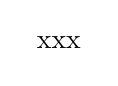
\begin{tikzpicture}
\node{xxx};
\end{tikzpicture}


Intuitivement, on peut "passer" d'un état à un autre soit en passant par une
arête "condition" qui s'évalue à une valeur "vrai", soit en appliquant les
effets de bord d'une arête "instruction".

Dans la suite, on suppose qu'on a à notre disposition un ensemble de jugements :
$\langle l, instr, l' \rangle$ qui signifie qu'on peut passer du point $l$ au
point $l'$ en effectuant l'instruction $instr$.

\subsection{État mémoire}
\label{sec:sigma}

L'interpréteur défini ici manipule des valeurs :

\gramlr{Valeurs}{
\begin{align*}
v  \gramisa  & n           & \textrm{Entier}
\\ \gramor   & f           & \textrm{Flottant}
\\ \gramor   & \cNil       & \textrm{Pointeur nul}
\\ \gramor   & \&a         & \textrm{Pointeur sur l'adresse $a$}
\\ \gramor   & \&f         & \textrm{Pointeur sur la fonction $f$}
\\ \gramor   & \top        & \textrm{Valeur non initialisée}
\end{align*}
}

On note l'ensemble des valeurs \textsc{Val}.

\begin{definition}[État mémoire]
L'interpréteur possède une mémoire, indexée par un ensemble d'adresses noté
\textsc{Addr}. Un état mémoire $σ$ est une fonction partielle de \textsc{Addr}
vers \textsc{Val}.
\end{definition}

\todo{Il faut une opération genre fromBytes}

\todo{Pile d'appels}

\begin{definition}[Fonction de transition]
La sémantique concrète que nous définissons ici est constituée de jugements
logiques. Le jugement principal est une relation de transition $\rightarrow$
entre états de l'interpréteur : il sera donc noté $Γ ⊢ (l, σ) \rightarrow (l', σ')$.
\end{definition}

\subsection{Jugements}

La sémantique concrète repose sur des jugements logiques et des règles
d'inférences, de la forme :

\[
\irule{Nom}{P_1 \\ … \\ P_n}{C}
\]

Les $P_i$ sont les prémisses, et $C$ la conclusion. Cette règle s'interprète de
la manière suivante : si les $P_i$ sont prouvées, alors $C$ est prouvée.

Certaines règles n'ont pas de prémisse : on parle alors d'axiome.

\[
\irule{Ax}{ }{A}
\]

Compte-tenu de la structure des règles, la preuve d'un jugement pourra donc être
vue sous la forme d'un arbre :

\[
  \irule{r1}{
    \irule{r2}
          {
            \irule{r3}
              { }
              {A_1}
              \\
            \irule{r4}
              { }
              {A_2}
          }
          {B_1}
    \\
    \irule{r5}
      {
        \irule{r6}
          { }
          {A_3}
        }{B_2}
      }{C}
\]

\subsection{Sémantique des left-values}

La mémoire est organisée en adresses, mais pourtant dans le programme cette
notion n'est pas directement visible. Les accès sont réalisés à travers des
"left values". Dans le langage C, elles correspondent aux constructions qui
peuvent se retrouver à gauche du signe "=" dans une affectation.

\begin{definition}[Correspondance left-values / adresses]
  Sous un environnement $Γ$ et un état mémoire $σ$, une left-value peut
  correspondre à une adresse $a$. Ceci sera noté $Γ, σ ⊢ lv ↝ a$.
\end{definition}

\begin{mathpar}
\irule{Eval-Lv-Var}{
  (v, a) ∈ σ
}{
  Γ, σ ⊢ v ↝ a
}
\and
\irule{Eval-Lv-Deref}{
  Γ, σ ⊢ e ⇒ \&a
}{
  Γ, σ ⊢ *e ↝ a
}
\and
\irule{Eval-Lv-Field}{
  Γ, σ ⊢ lv ↝ a
}{
  Γ, σ ⊢ lv.f ↝ a + f
}
\and
\irule{Eval-Lv-Array}{
  Γ, σ ⊢ lv ↝ a \\
  Γ, σ ⊢ e ⇒ n
}{
  Γ, σ ⊢ lv[e] ↝ a + n
}
\end{mathpar}

\subsection{Sémantique des expressions}

\begin{definition}[Évaluation d'une expression]
  Sous un environnement $Γ$ et un état mémoire $σ$, une left-value peut
  produire une valeur $v$. Ceci sera noté $Γ, σ ⊢ e ⇒ v$.
\end{definition}

Dans le cas où l'expression est une constante, c'est directement le résultat.

\begin{mathpar}
\irule{Eval-Cst}{
}{
  Γ, σ ⊢ c ⇒ c
}
\end{mathpar}

Si l'expression est une left-value, on établit à quelle adresse elle correspond
et on récupère dans l'état mémoire à quelle valeur celle-ci correspond.

\begin{mathpar}
\irule{Eval-Lv}{
  Γ, σ ⊢ lv ↝ a \\
  (a, v) ∈ σ
}{
  Γ, σ ⊢ lv ⇒ v
}
\end{mathpar}

En ce qui concerne les opérations (unaires ou binaires), on commence par évaluer
les opérandes. Le résultat est l'opération "concrète" sur les valeurs, notée
$\widehat{\textrm{op}}$. Par exemple, pour la construction syntaxique $+$, on
utilise l'addition sur les valeurs $\widehat{+}$ (c'est-à-dire l'addition
usuelle).

\begin{mathpar}
\irule{Eval-Unop}{
  Γ, σ ⊢ e ⇒ v
}{
  Γ, σ ⊢ \textrm{op}~e ⇒ \widehat{\textrm{op}}~v
}
\and
\irule{Eval-Binop}{
  Γ, σ ⊢ e_1 ⇒ v_1 \\
  Γ, σ ⊢ e_2 ⇒ v_2
}{
  Γ, σ ⊢ e_1~\textrm{op}~e_2 ⇒ v_1~\widehat{\textrm{op}}~v_2
}
\end{mathpar}

Enfin, les adresses sont aussi des valeurs. Le cas des pointeurs sur fonction
est direct puisque toutes les fonctions sont globales ; pour le cas des
pointeurs sur données on commence par déterminer l'adresse de l'objet pointé
depuis l'état mémoire.

\begin{mathpar}
\irule{Eval-AddrOfFun}{
}{
  Γ, σ ⊢ \&f ⇒ \&f
}
\and
\irule{Eval-AddrOf}{
  Γ, σ ⊢ lv ↝ a
}{
  Γ, σ ⊢ \&lv ⇒ \&a
}
\end{mathpar}

\subsection{Sémantique des instructions}

La règle la plus simple concerne l'affectation : on peut affecter une
expressions à une left value si elles ont le même type.

\begin{mathpar}
  \irule{Instr-Assign}{
    \langle l, lv \leftarrow e, l' \rangle \\
    Γ, σ ⊢ lv ↝ a \\
    Γ, σ ⊢ e ⇒ v
  }{
    Γ ⊢ (l, σ) \rightarrow (l', σ [ a ↦ v ])
  }
\end{mathpar}

Déclarer une variable, c'est rendre accessible dans un bloc une variable non
initialisée, qui n'est plus accessible par la suite : Si on suppose qu'on peut
traverser le bloc interne $b$ sous un $σ$ enrichi d'une nouvelle variable $x$,
on peut donc traverser l'instruction \npkDecl{x}{b}.

\begin{minipage}{0.6\textwidth}
\begin{mathpar}
  \irule{Instr-Decl}{
    \langle l, \npkDecl{x}{b}, l' \rangle \\
    \langle l_b, b, l_b' \rangle \\
    σ' = σ ⊕ \{ x \rightarrow \top \} \\
    Γ ⊢ (l_b, σ', s) \rightarrow (l_b', σ'')
  }{
    Γ ⊢ (l, σ) \rightarrow (l', σ'' \backslash x)
  }
\end{mathpar}
\end{minipage}
\begin{minipage}{0.4\textwidth}
\begin{tikzpicture}
  [cfgnode/.style={draw,shape=circle},node distance=2cm]
  \node[cfgnode] (l) {$l$};
  \node[cfgnode,right of=l, node distance=4cm] (lp) {$l'$};
  \node[cfgnode,below of=l, xshift=1cm] (lb) {$l_b$};
  \node[cfgnode,below of=lp, xshift=-1cm] (lbp) {$l_b'$};
  \draw[->] (l)  to node[auto] {$↑x\{b\}$} (lp);
  \draw[->] (lb) to node[auto] {$b$} (lbp);
  \draw[->,dashed] (l) to node[auto] {$⊕ \{ x → \top \}$}(lb);
  \draw[->,dashed,swap] (lbp) to node[auto] {$\backslash x$} (lp);
\end{tikzpicture}

\end{minipage}

\todo{fcall}

TODO pour :

\[
\irule{Instr-Fcall}{
  \langle l, lv \leftarrow fe(\vec{e}), l' \rangle \\
  σ ⊢ fe ⇒ f \\
  Γ, σ ⊢ \vec{e} ⇒ \vec{v} \\
  σ' = σ ⊕ \{args(f) = \vec{v}\} ⊕ \{ !ret \rightarrow \top \} \\
  Γ ⊢ (Entry(f), σ') \rightarrow (Exit(f), σ'') \\
  Γ, σ'' ⊢ !ret ⇒ v_{ret} \\
  Γ, σ'' ⊢ lv ↝ a
}{
  Γ ⊢ (l, σ) \rightarrow (l', σ'' \backslash (args(f) \cup \{!ret\}) ⊕ \{ a \rightarrow v_{ret}\}, ?)
}
\]

\todo{definir $σ ⊢ fe ⇒ f$}

\subsection{Sémantique des conditions}

On utilise un encodage similaire à la déclaration. Tout d'abord, on évalue la
condition dans un contexte $σ$. Si elle s'évalue en un entier non nul, et qu'une
transition à travers le bloc $i_t$ est possible, alors on peut faire passer à
travers le "\textsc{If}".

\begin{minipage}{0.5\textwidth}
\begin{tikzpicture}
  [cfgnode/.style={draw,shape=circle}, node distance=1.5cm]
  \node[cfgnode] (l) {$l$};
  \node[cfgnode,right of=l, node distance=4.5cm] (lp) {$l'$};
  \node[cfgnode,below of=l, xshift=5mm] (lt) {$l_t$};
  \node[cfgnode,below of=lp, xshift=-5mm] (ltp) {$l_t'$};
  \node[cfgnode,above of=l, xshift=5mm] (lf) {$l_f$};
  \node[cfgnode,above of=lp, xshift=-5mm] (lfp) {$l_f'$};
  \draw[->] (l)  to node[auto] {$\npkIf{e}{i_t}{i_f}$} (lp);
  \draw[->] (lt) to node[auto] {$i_t$} (ltp);
  \draw[->] (lf) to node[auto] {$i_f$} (lfp);
  \draw[->,dashed] (l) to node [auto,swap] {$≠0$} (lt);
  \draw[->,dashed] (ltp) to (lp);
  \draw[->,dashed] (l) to node [auto] {$0$} (lf);
  \draw[->,dashed] (lfp) to (lp);
\end{tikzpicture}

\end{minipage}
\begin{minipage}{0.5\textwidth}
\begin{mathpar}
\irule{If-True}{
  \langle l, \npkIf{e}{i_t}{i_f}, l' \rangle \\
  Γ, σ ⊢ e ⇒ n \\
  n ≠ 0 \\
  \langle l_i, i_t, l_i' \rangle \\
  Γ ⊢ (l_i, σ) \rightarrow (l_i', σ')
}{
  Γ ⊢ (l, σ) \rightarrow (l', σ')
}
\and
\irule{If-False}{
  \langle l, \npkIf{e}{i_t}{i_f}, l' \rangle \\
  Γ, σ ⊢ e ⇒ 0 \\
  \langle l_i, i_f, l_i' \rangle \\
  Γ ⊢ (l_i, σ) \rightarrow (l_i', σ')
}{
  Γ ⊢ (l, σ) \rightarrow (l', σ')
}
\end{mathpar}
\end{minipage}

\section{Règles de typage}

\subsection{Types}

Dans cette section, on définit la notion de programme bien typé. L'analyse par
typage permet de vérifier qu'à chaque expression on peut associer un type, et ce
de manière cohérente entre plusieurs utilisations d'une variable.

Les types des valeurs sont :

\gramlr{Types}{
\begin{align*}
τ  \gramisa & \tInt, \tFloat, \tVoid        & \textrm{Constante}
\\ \gramor  &  a                            & \textrm{Variable}
\\ \gramor  & (τ_1, …, τ_n) \rightarrow τ_r & \textrm{Fonction}
\\ \gramor  & [τ]                           & \textrm{Tableau}
\\ \gramor  & τ*                            & \textrm{Pointeur}
\\ \gramor  & \{ f_1:τ_1
              ,    …
              , f_n:τ_n \}                  & \textrm{Structure}
\end{align*}
}

L'ensemble des types possibles (défini inductivement ci-dessus) sera noté
\textsc{Typ}, et l'ensemble des variables de type par \textsc{VarTyp}.

\subsection{Schémas de type}

On va associer à chaque variable globale un type. Mais faire de même pourrait
être trop restrictif. En effet, une fonction comme memcpy peut être utilisée
pour copier des tableaux d'entiers, mais aussi de flottants. On va donc associer
un schéma de types à chaque fonction.

\gramlr{Schémas}{
\begin{align*}
σ \gramisa & ∀ \vec{a} . τ
\end{align*}
}

Un schéma de types correspond à un ensemble de types. Prenons l'exemple de la
fonction identité : elle a pour schéma de types $∀ a . a \rightarrow a$, ce qui
signifie que pour chaque type $τ$, on peut l'utiliser avec le type $τ
\rightarrow τ$. Plus précisément, cela veut dire que puisque $a$ est quantifiée,
on peut le substituer par n'importe quel autre type.

\begin{definition}[Substitution]
Une substitution est une fonction partielle de \textsc{VarTyp} dans
\textsc{Typ}. Elle sera notée par exemple $s = \{ a ↦ \tInt, b ↦ (\tFloat
\rightarrow \tInt)\}$.

Le support d'une substition, noté $\textrm{Supp}(s)$, est son domaine de
définition.

On définit aussi l'application d'une substitution sur un type quelconque : si
$s$ est une substitution, $\overline{s}$ est son extension définie par :

\begin{align*}
\overline{s}(a)   =~& s(a) & \textrm{si $a$ est une variable}  \\
\overline{s}(c)   =~& c    & \textrm{si $c$ est une constante} \\
\overline{s}([τ]) =~& [\overline{s}(τ)] & \\
\overline{s}(τ*)  =~& \overline{s}(τ)*   & \\
\overline{s}(τ_1, …, τ_n) \rightarrow τ_r =~& (\overline{s}(τ_1), …, \overline{s}(τ_n)) \rightarrow \overline{s}(τ_r) \\
\overline{s}(\{ f_1:τ_1, … ,f_n:τ_n \}) =~& \{ f_1:\overline{s}(τ_1), …, f_n:\overline{s}(τ_n) \}
\end{align*}

Par souci de simplicité, on notera $s$ pour $\overline{s}$.
\end{definition}

\begin{definition}[Instanciation]
Un schéma de types $σ = ∀ \vec{a} . τ$ peut être instancié en un type $μ$ s'il
existe une substition $s$ telle que :

\begin{itemize}
\item $\textrm{Supp}(s) ⊆ \vec{a}$
\item $s(τ) = μ$
\end{itemize}

On note alors $μ ≤ σ$.
\end{definition}

\begin{definition}[Variables libres]
Les variables libres d'un type sont l'ensemble des variables de types qui
apparaissent dans celui-ci :

\begin{align*}
\tFV{a}   =~& ∅    & \textrm{si $a$ est une variable}  \\
\tFV{c}   =~& ∅    & \textrm{si $c$ est une constante} \\
\tFV{[τ]} =~& \tFV{τ} & \\
\tFV{τ*}  =~& \tFV{τ} & \\
\tFV{(τ_1, …, τ_n) \rightarrow τ_r} =~& \tFV{τ_1} ∪ … ∪ \tFV{τ_n} ∪ \tFV{τ_r} \\
\tFV{\{ f_1:τ_1, … ,f_n:τ_n \}} =~& \tFV{τ_1} ∪ … ∪ \tFV{τ_n}
\end{align*}
\end{definition}

\begin{definition}[Généralisation]
La généralisation consiste à construire un schéma de type à partir d'un type, en
quantifiant sur les variables libres :

\[
\textrm{Gen}(τ) = ∀ \vec{a} . τ \quad \textrm{où} \quad \vec{a} = \tFV{τ}
\]
\end{definition}

En associant un schéma de type $σ$ à une fonction $f$, on indique que la
fonction pourra être utilisée avec tout type $τ$ qui est une instanciation de
$σ$.

\subsection{Environnements de typage}

Chaque jugement de typage est effectué dans un environnement de typage $Γ$
particulier, qui contient le contexte nécessaire : ici, le type des fonctions et
variables du programme.

\gramlr{Environnements}{
\begin{align*}
Γ  \gramisa & (Γ_{fun}, Γ_{var}) & \textrm{Fonctions, variables}
\end{align*}

\begin{align*}
Γ_{fun} \gramisa & ε           & \textrm{Environnement vide}
\\      \gramor  & Γ_{fun},f:σ & \textrm{Ajout d'une fonction}
\end{align*}

\begin{align*}
Γ_{var} \gramisa & ε           & \textrm{Environnement vide}
\\      \gramor  & Γ_{var},v:τ & \textrm{Ajout d'une variable}
\end{align*}
}

Lorsque ce n'est pas ambigü, si $Γ=(Γ_{fun},Γ_{var})$ on notera les extensions
d'environnement $Γ,f:σ$ pour $((Γ_{fun},f:σ), Γ_{var})$ et $Γ,x:τ$ pour
$(Γ_{fun},(Γ_{var},x:τ))$. De même, on notera $(f, σ) ∈ Γ$ si $(f, σ) ∈
Γ_{fun}$, ou $(x, τ) ∈ Γ$ si $(x, τ) ∈ Γ_{var}$.

\subsection{Jugements de typage}

\begin{definition}[Jugement de typage]
Un jugement de typage est de la forme $Γ ⊢ e : τ$ et se lit "sous $Γ$, $e$ est
typable en $τ$".
\end{definition}

\begin{definition}[Bloc bien typé]
Les instructions et blocs, au contraire, n'ont pas de type. On note $Γ ⊢ i$ pour
"sous $Γ$, $i$ est bien typé", c'est à dire que ces sous expressions sont
typables en accord avec le flot de données (par exemple, pour que l'instruction
$lv \leftarrow e$ soit bien typée sous $Γ$, il faut que les types de $lv$ et de
$e$ puissent avoir le même type sous $Γ$).
\end{definition}

\begin{definition}[Fonction bien typée]
…
\end{definition}

\begin{definition}[Programme bien typé]
Un programme $P$ est bien typé s'il existe un environnement $Γ$ permettant de bien
typer toutes les composantes (fonctions, globales et bloc d'initialisation) d'un
programme. On notera alors $⊢ P$.
\end{definition}

\subsection{Programme}

Au niveau global, un programme P est bien typé (noté $⊢ P$) s'il existe un
environnement $Γ = (\vec{σ}, \vec{τ})$ permettant de typer ses composantes (les fonctions, les
globales et le bloc d'initialisation).

\[
\irule{Prog}{
  (\vec{σ}, \vec{τ}) ⊢ \vec{f} : \vec{σ} \\
  (\vec{σ}, \vec{τ}) ⊢ \vec{x} : \vec{t} \\
  (\vec{σ}, \vec{τ}) ⊢ b
}{
  ⊢ (\vec{f}, \vec{x}, b)
}
\]

\subsection{Flot de contrôle}

Les règles suivantes permettent de définir les jugements $Γ ⊢ i$. De manière
générale, les instructions sont bien typées si leurs sous-instructions sont bien typées.

\begin{mathpar}
\irule{Pass}{
}{
  Γ ⊢ ε
}
\and
\irule{Seq}{
  Γ ⊢ s \\
  Γ ⊢ b
}{
  Γ ⊢ s;b
}
\and
\irule{While}{
  Γ ⊢ b
}{
  Γ ⊢ \npkWhile{b}
}
\and
\irule{Goto}{
}{
  Γ ⊢ \npkGoto{l}
}
\and
\irule{DoWith}{
  Γ ⊢ b
}{
  Γ ⊢ \npkDoWith{b}{l}
}
\end{mathpar}

Dans le cas de la conditionnelle, il est en plus nécessaire de vérifier que la
condition est un entier.

\begin{mathpar}
\irule{If}{
  Γ ⊢ e : \tInt \\
  Γ ⊢ i_t \\
  Γ ⊢ i_f
}{
  Γ ⊢ \npkIf{e}{i_t}{i_f}
}
\end{mathpar}

\subsection{Left values}

On associe à chaque left-value un type, qui est aussi le type des valeurs que
celle-ci peut contenir. Le cas des variables est direct : si un couple
(variable, type) est dans l'environnement de typage, la variable possède ce
type.

\begin{mathpar}
\irule{Lv-Var}{
  (v, τ) ∈ Γ
}{
  Γ ⊢ v : τ
}
\end{mathpar}

Si une expression a un type pointeur, en la déréférençant on obtient une valeur
du type pointé.

\begin{mathpar}
\irule{Lv-Deref}{
  Γ ⊢ e : τ*
}{
  Γ ⊢ *e : τ
}
\end{mathpar}

\todo{accès à un élément d'un type composite}

\begin{mathpar}
\irule{Lv-Field}{
  Γ ⊢ lv : τ_s \\
  (f, τ_f) ∈ τ_s
}{
  Γ ⊢ lv.f : τ_f
}
\and
\irule{Lv-Array}{
  Γ ⊢ lv : [τ] \\
  Γ ⊢ e : \tInt
}{
  Γ ⊢ lv[e] : τ
}
\end{mathpar}

\subsection{Expressions}

Les constantes ont leurs types habituels. Notons que le pointeur nul (\cNil) a
un type polymorphe.

\begin{mathpar}
\irule{Const-Int}{
}{
  Γ ⊢ n : \tInt
}
\and
\irule{Const-Float}{
}{
  Γ ⊢ f : \tFloat
}
\and
\irule{Const-Nil}{
}{
  Γ ⊢ \cNil : τ*
}
\end{mathpar}

Un certain nombre d'opérations est possible sur le type \tInt.

\begin{mathpar}
\irule{Op-Int}{
  \textrm{op} ∈ \{+,-,\times,/,\&,|,\opxor,\&\&,||,⋘,⋙\} \\
  Γ ⊢ e_1 : \tInt \\
  Γ ⊢ e_2 : \tInt
}{
  Γ ⊢ e_1~\textrm{op}~e_2 : \tInt
}
\end{mathpar}

De même sur \tFloat.

\begin{mathpar}
\irule{Op-Float}{
  \textrm{op} ∈ \{+.,-.,\times.,/.\} \\
  Γ ⊢ e_1 : \tFloat \\
  Γ ⊢ e_2 : \tFloat
}{
  Γ ⊢ e_1~\textrm{op}~e_2 : \tFloat
}
\end{mathpar}

Les opérateurs de comparaison peuvent s'appliquer à deux opérandes de types
\tInt ou \tFloat et renvoient un \tInt.

\begin{mathpar}
\irule{Op-Cmp}{
  \textrm{op} ∈ \{=,≠,≤,≥,<,>\} \\
  Γ ⊢ e_1 : τ \\
  Γ ⊢ e_2 : τ \\
  τ ∈ \{ \tInt, \tFloat \}
}{
  Γ ⊢ e_1~\textrm{op}~e_2 : \tInt
}
\end{mathpar}

L'opérateur unaire $-$ peut être appliqué à un \tInt ou à un \tFloat.

\begin{mathpar}
\irule{Unop-Minus}{
  τ ∈ \{ \tInt, \tFloat \} \\
  Γ ⊢ e : τ
}{
  Γ ⊢ -e : τ
}
\end{mathpar}

Les opérateurs de négation unaires, en revanche, ne s'appliquent qu'aux
entiers.

\begin{mathpar}
\irule{Unop-Not}{
  \textrm{op} ∈ \{ \textasciitilde, ! \} \\
  Γ ⊢ e : \tInt
}{
  Γ ⊢ \textrm{op}~e : \tInt
}
\end{mathpar}

On peut prendre l'adresse d'une left-value, et obtenir un pointeur vers
celle-ci. Le type du résultat est un type pointeur vers le type de base.

\begin{mathpar}
\irule{AddrOf}{
  Γ ⊢ lv : τ
}{
  Γ ⊢ \&lv : τ*
}
\end{mathpar}

La règle concernant les pointeurs sur fonction est similaire, à ceci près que
les fonctions ont des schémas de type. Un pointeur sur fonction peut donc avoir
n'importe quelle instanciation de ce schéma.

\begin{mathpar}
\irule{AddrOfFun}{
  Γ ⊢ f : σ \\
  τ ≤ σ
}{
  Γ ⊢ \&lv : τ
}
\end{mathpar}

\subsection{Fonctions}

Pour typer une fonction, on commence par ajouter ses paramètres dans
l'environnement de typage, et on type la définition de la fonction. Le type
résultant est généralisé.

\todo{Vérifier qu'il n'y a pas de problème entre polymorphisme et mutabilité}

\todo{Notation vecteur}

\[
\irule{Fun}{
  Γ' = Γ ⊕ \{ args(f) = \vec{τ} \} \\
  Γ' ⊢ body(f) \\
  Γ' ⊢ !ret : τ_r
}{
  Γ ⊢ f : Gen(\vec{τ} \rightarrow τ_r, Γ)
}
\]

\subsection{Instructions}

\begin{mathpar}
\irule{Decl}{
  Γ ⊕ \{x : τ\} ⊢ b
}{
  Γ ⊢ \npkDecl{x}{b}
}
\and
\irule{Assign}{
  Γ ⊢ lv : τ \\
  Γ ⊢ e  : τ
}{
  Γ ⊢ lv \leftarrow e
}
\and
\irule{Fcall}{
  Γ ⊢ lv : τ_{ret} \\
  Γ ⊢ fe : σ \\
  Γ ⊢ \vec{e} : \vec{τ} \\
  (\vec{τ} \rightarrow τ_r) ≤ σ
}{
  Γ ⊢ lv \leftarrow fe(\vec{e})
}
\end{mathpar}

\section{Limitations}
\subsection{Programmes non typables}
\subsection{Incohérences}
